\documentclass[a4paper,12pt]{article}
\usepackage[utf8]{inputenc}
\usepackage[french]{babel}
\usepackage{geometry}
\usepackage{titlesec}
\usepackage{hyperref}
\usepackage{enumitem}
\usepackage{float}
\usepackage{graphicx}
\geometry{margin=2.5cm}
\titleformat{\section}{\large\bfseries}{\thesection.}{1em}{}


\title{Implémentation d’un réseau d’école avec Cisco Packet Tracer}
\author{MBOLANIRINA Stephano Kevin\\Sous la direction de Mr Andriamanjaka}
\date{}

\begin{document}

\maketitle
\newpage
\tableofcontents
\newpage

\section{Présentation générale du projet}
Ce projet consiste à créer un parc réseau informatique dans une école. Le principal but est que chaque entité personnelle ait accès au réseau en général et accéder ou non à certaines fonctionnalités dans le réseau.

\section{Description de l’environnement}

\subsection{Topologie}
\begin{figure}[H]
    \centering
    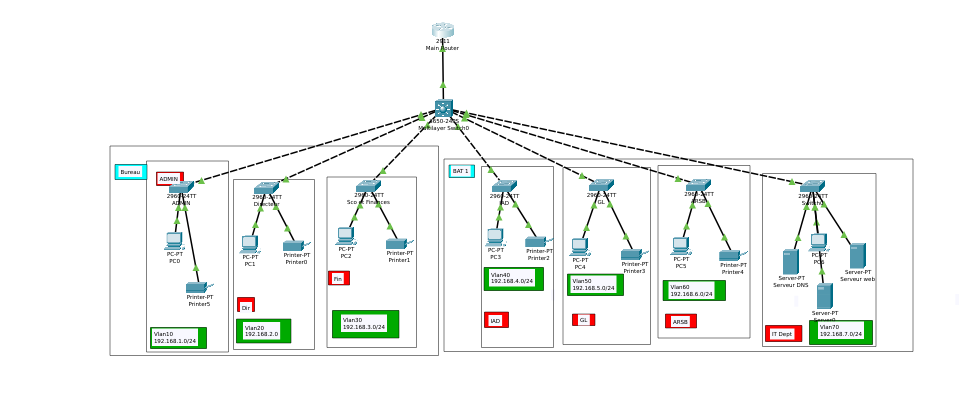
\includegraphics[width=1.2\textwidth]{CAPTURE/Top.png}
    \caption{}
    \label{fig:snort_install}
\end{figure}

Selon cette topologie, on a deux bâtiments principaux : celui qui contient les bureaux et celui qui contient les salles de classe où les élèves étudient, ainsi que la salle qui contient les serveurs nécessaires pour le bon fonctionnement de l’école.

\begin{itemize}
    \item \textbf{Couche d'accès} : connecte directement les terminaux (PC, imprimantes, serveurs). Chaque département dispose d’un switch d’accès.
    \item \textbf{Couche de distribution} : agrège le trafic provenant des switches d’accès et permet le routage inter-VLAN.
    \item \textbf{Couche cœur} : s’occupe du transfert rapide des données vers d'autres sites ou Internet.
\end{itemize}

\section{Technologie à utiliser}

\subsection{VLAN}
Un VLAN (Virtual Local Area Network) est un sous-réseau logique créé à l'intérieur d’un réseau physique. Il permet de regrouper des appareils selon leur fonction, département ou niveau de sécurité.

\subsection{Configuration de chaque VLAN}
Pour notre projet, nous aurons besoin de 7 VLAN :

\begin{itemize}
    \item VLAN 10 : Administrateurs réseau
    \item VLAN 20 : Direction
    \item VLAN 30 : Branche Finance
    \item VLAN 40 : Département IAD
    \item VLAN 50 : Département GL
    \item VLAN 60 : Département ARSB
    \item VLAN 70 : Département IT
\end{itemize}

\textbf{\\Sur les switches d'accès :}
\begin{verbatim}
int range Fa0/1-24
switchport mode access
switchport access vlan {numéro du vlan}
\end{verbatim}

\textbf{Sur les switches de distribution (exemple pour VLAN 10) :}
\begin{verbatim}
int Gig1/0/1
switchport mode access
switchport access vlan 10
\end{verbatim}
.\\On fait les mêmes commandes pour chaque interface du switch pour tout les VLAN. 

\section{Besoins techniques}

\subsection{Mode Trunk}
Pour que les informations, les données, et les paquets puissent transiter dans le réseau, l’interface du switch de niveau 3 reliée au routeur doit être en mode trunk :
\begin{verbatim}
int gig1/0/1
switchport trunk encapsulation dot1q
switchport mode trunk
\end{verbatim}

\subsection{Création des sous-interfaces pour chaque VLAN}
.\\
La création des sous-interfaces pour chaque VLAN se passe au niveau du routeur (couche
cœur). Voici la table d'adressage
\begin{center}
\begin{tabular}{|c|c|c|}
\hline
Interface & VLAN & Adresse IP \\
\hline
Gig0/0.10 & VLAN 10 & 192.168.1.1/24 \\
Gig0/0.20 & VLAN 20 & 192.168.2.1/24 \\
Gig0/0.30 & VLAN 30 & 192.168.3.1/24 \\
Gig0/0.40 & VLAN 40 & 192.168.4.1/24 \\
Gig0/0.50 & VLAN 50 & 192.168.5.1/24 \\
Gig0/0.60 & VLAN 60 & 192.168.6.1/24 \\
Gig0/0.70 & VLAN 70 & 192.168.7.1/24 \\
\hline
\end{tabular}
\end{center}

\textbf{Exemple de configuration (VLAN 10) :}
\begin{verbatim}
interface GigabitEthernet0/0.10
encapsulation dot1Q 10
ip address 192.168.1.1 255.255.255.0
no shutdown
\end{verbatim}

\subsection{Configuration du serveur DHCP}
.\\Un serveur DHCP (Dynamic Host Configuration Protocol) est un serveur réseau qui attribue
automatiquement des adresses IP et d’autres paramètres de configuration réseau aux appareils
(clients) qui se connectent à un réseau.
.\\On peut configurer directement un serveur DHCP au niveau du routeur avec les commandes (pour VLAN 10 par exemple):
\begin{verbatim}
service dhcp
dhcp pool Admin-pool
network 192.168.1.0 255.255.255.0
default-router 192.168.1.1
dns-server 192.168.1.1
exit
\end{verbatim}
.\\On fait les mêmes commandes pour tout les VLAN.\\

\textit{Remarque : les serveurs doivent avoir une adresse IP statique.}

\subsection{Création des filtrages par utilisateurs (ACL)}
Pour les filtrages, nous allons utiliser un \textbf{ACL}.
Une ACL (Access Control List ou liste de contrôle d’accès) est un ensemble de règles utilisées
pour contrôler l’accès à des ressources informatiques, telles que des fichiers, des applications
ou des réseaux .\\

Dans notre besoin, seuls les VLAN 10, 20, et 30 peuvent accéder au serveur FTP (192.168.7.10). Les VLAN 40, 50, 60 sont bloqués.

\textbf{Exemple de configuration ACL :}
\begin{verbatim}
ip access-list extended BLOCK_FTP

deny tcp 192.168.4.0 0.0.0.255 host 192.168.7.10 eq 21
deny tcp 192.168.5.0 0.0.0.255 host 192.168.7.10 eq 21
deny tcp 192.168.6.0 0.0.0.255 host 192.168.7.10 eq 21
permit ip any any
\end{verbatim}

\textbf{Application de l’ACL sur l’interface VLAN 70 :} l'ACL doit être appliquée en entrée sur l’interface VLAN70 du routeur, c’est-à-dire avant
que le trafic atteigne le serveur FTP :
\begin{verbatim}
interface GigabitEthernet0/0.70
ip access-group BLOCK_FTP in
\end{verbatim}

\textit{Ainsi, les étudiants ne pourront pas accéder au serveur FTP.}

\end{document}
